% Options for packages loaded elsewhere
\PassOptionsToPackage{unicode}{hyperref}
\PassOptionsToPackage{hyphens}{url}
%
\documentclass[
  12pt,
]{article}
\usepackage{amsmath,amssymb}
\usepackage{iftex}
\ifPDFTeX
  \usepackage[T1]{fontenc}
  \usepackage[utf8]{inputenc}
  \usepackage{textcomp} % provide euro and other symbols
\else % if luatex or xetex
  \usepackage{unicode-math} % this also loads fontspec
  \defaultfontfeatures{Scale=MatchLowercase}
  \defaultfontfeatures[\rmfamily]{Ligatures=TeX,Scale=1}
\fi
\usepackage{lmodern}
\ifPDFTeX\else
  % xetex/luatex font selection
  \setmainfont[]{Times New Roman}
\fi
% Use upquote if available, for straight quotes in verbatim environments
\IfFileExists{upquote.sty}{\usepackage{upquote}}{}
\IfFileExists{microtype.sty}{% use microtype if available
  \usepackage[]{microtype}
  \UseMicrotypeSet[protrusion]{basicmath} % disable protrusion for tt fonts
}{}
\makeatletter
\@ifundefined{KOMAClassName}{% if non-KOMA class
  \IfFileExists{parskip.sty}{%
    \usepackage{parskip}
  }{% else
    \setlength{\parindent}{0pt}
    \setlength{\parskip}{6pt plus 2pt minus 1pt}}
}{% if KOMA class
  \KOMAoptions{parskip=half}}
\makeatother
\usepackage{xcolor}
\usepackage[margin=1in]{geometry}
\usepackage{color}
\usepackage{fancyvrb}
\newcommand{\VerbBar}{|}
\newcommand{\VERB}{\Verb[commandchars=\\\{\}]}
\DefineVerbatimEnvironment{Highlighting}{Verbatim}{commandchars=\\\{\}}
% Add ',fontsize=\small' for more characters per line
\usepackage{framed}
\definecolor{shadecolor}{RGB}{248,248,248}
\newenvironment{Shaded}{\begin{snugshade}}{\end{snugshade}}
\newcommand{\AlertTok}[1]{\textcolor[rgb]{0.94,0.16,0.16}{#1}}
\newcommand{\AnnotationTok}[1]{\textcolor[rgb]{0.56,0.35,0.01}{\textbf{\textit{#1}}}}
\newcommand{\AttributeTok}[1]{\textcolor[rgb]{0.13,0.29,0.53}{#1}}
\newcommand{\BaseNTok}[1]{\textcolor[rgb]{0.00,0.00,0.81}{#1}}
\newcommand{\BuiltInTok}[1]{#1}
\newcommand{\CharTok}[1]{\textcolor[rgb]{0.31,0.60,0.02}{#1}}
\newcommand{\CommentTok}[1]{\textcolor[rgb]{0.56,0.35,0.01}{\textit{#1}}}
\newcommand{\CommentVarTok}[1]{\textcolor[rgb]{0.56,0.35,0.01}{\textbf{\textit{#1}}}}
\newcommand{\ConstantTok}[1]{\textcolor[rgb]{0.56,0.35,0.01}{#1}}
\newcommand{\ControlFlowTok}[1]{\textcolor[rgb]{0.13,0.29,0.53}{\textbf{#1}}}
\newcommand{\DataTypeTok}[1]{\textcolor[rgb]{0.13,0.29,0.53}{#1}}
\newcommand{\DecValTok}[1]{\textcolor[rgb]{0.00,0.00,0.81}{#1}}
\newcommand{\DocumentationTok}[1]{\textcolor[rgb]{0.56,0.35,0.01}{\textbf{\textit{#1}}}}
\newcommand{\ErrorTok}[1]{\textcolor[rgb]{0.64,0.00,0.00}{\textbf{#1}}}
\newcommand{\ExtensionTok}[1]{#1}
\newcommand{\FloatTok}[1]{\textcolor[rgb]{0.00,0.00,0.81}{#1}}
\newcommand{\FunctionTok}[1]{\textcolor[rgb]{0.13,0.29,0.53}{\textbf{#1}}}
\newcommand{\ImportTok}[1]{#1}
\newcommand{\InformationTok}[1]{\textcolor[rgb]{0.56,0.35,0.01}{\textbf{\textit{#1}}}}
\newcommand{\KeywordTok}[1]{\textcolor[rgb]{0.13,0.29,0.53}{\textbf{#1}}}
\newcommand{\NormalTok}[1]{#1}
\newcommand{\OperatorTok}[1]{\textcolor[rgb]{0.81,0.36,0.00}{\textbf{#1}}}
\newcommand{\OtherTok}[1]{\textcolor[rgb]{0.56,0.35,0.01}{#1}}
\newcommand{\PreprocessorTok}[1]{\textcolor[rgb]{0.56,0.35,0.01}{\textit{#1}}}
\newcommand{\RegionMarkerTok}[1]{#1}
\newcommand{\SpecialCharTok}[1]{\textcolor[rgb]{0.81,0.36,0.00}{\textbf{#1}}}
\newcommand{\SpecialStringTok}[1]{\textcolor[rgb]{0.31,0.60,0.02}{#1}}
\newcommand{\StringTok}[1]{\textcolor[rgb]{0.31,0.60,0.02}{#1}}
\newcommand{\VariableTok}[1]{\textcolor[rgb]{0.00,0.00,0.00}{#1}}
\newcommand{\VerbatimStringTok}[1]{\textcolor[rgb]{0.31,0.60,0.02}{#1}}
\newcommand{\WarningTok}[1]{\textcolor[rgb]{0.56,0.35,0.01}{\textbf{\textit{#1}}}}
\usepackage{longtable,booktabs,array}
\usepackage{calc} % for calculating minipage widths
% Correct order of tables after \paragraph or \subparagraph
\usepackage{etoolbox}
\makeatletter
\patchcmd\longtable{\par}{\if@noskipsec\mbox{}\fi\par}{}{}
\makeatother
% Allow footnotes in longtable head/foot
\IfFileExists{footnotehyper.sty}{\usepackage{footnotehyper}}{\usepackage{footnote}}
\makesavenoteenv{longtable}
\usepackage{graphicx}
\makeatletter
\def\maxwidth{\ifdim\Gin@nat@width>\linewidth\linewidth\else\Gin@nat@width\fi}
\def\maxheight{\ifdim\Gin@nat@height>\textheight\textheight\else\Gin@nat@height\fi}
\makeatother
% Scale images if necessary, so that they will not overflow the page
% margins by default, and it is still possible to overwrite the defaults
% using explicit options in \includegraphics[width, height, ...]{}
\setkeys{Gin}{width=\maxwidth,height=\maxheight,keepaspectratio}
% Set default figure placement to htbp
\makeatletter
\def\fps@figure{htbp}
\makeatother
\setlength{\emergencystretch}{3em} % prevent overfull lines
\providecommand{\tightlist}{%
  \setlength{\itemsep}{0pt}\setlength{\parskip}{0pt}}
\setcounter{secnumdepth}{5}
% definitions for citeproc citations
\NewDocumentCommand\citeproctext{}{}
\NewDocumentCommand\citeproc{mm}{%
  \begingroup\def\citeproctext{#2}\cite{#1}\endgroup}
\makeatletter
 % allow citations to break across lines
 \let\@cite@ofmt\@firstofone
 % avoid brackets around text for \cite:
 \def\@biblabel#1{}
 \def\@cite#1#2{{#1\if@tempswa , #2\fi}}
\makeatother
\newlength{\cslhangindent}
\setlength{\cslhangindent}{1.5em}
\newlength{\csllabelwidth}
\setlength{\csllabelwidth}{3em}
\newenvironment{CSLReferences}[2] % #1 hanging-indent, #2 entry-spacing
 {\begin{list}{}{%
  \setlength{\itemindent}{0pt}
  \setlength{\leftmargin}{0pt}
  \setlength{\parsep}{0pt}
  % turn on hanging indent if param 1 is 1
  \ifodd #1
   \setlength{\leftmargin}{\cslhangindent}
   \setlength{\itemindent}{-1\cslhangindent}
  \fi
  % set entry spacing
  \setlength{\itemsep}{#2\baselineskip}}}
 {\end{list}}
\usepackage{calc}
\newcommand{\CSLBlock}[1]{\hfill\break\parbox[t]{\linewidth}{\strut\ignorespaces#1\strut}}
\newcommand{\CSLLeftMargin}[1]{\parbox[t]{\csllabelwidth}{\strut#1\strut}}
\newcommand{\CSLRightInline}[1]{\parbox[t]{\linewidth - \csllabelwidth}{\strut#1\strut}}
\newcommand{\CSLIndent}[1]{\hspace{\cslhangindent}#1}
\usepackage{tcolorbox}
\usepackage{amssymb}
\usepackage{yfonts}
\usepackage{bm}

\newtcolorbox{greybox}{
  colback=white,
  colframe=blue,
  coltext=black,
  boxsep=5pt,
  arc=4pt}
  
\newcommand{\ds}[4]{\sum_{{#1}=1}^{#3}\sum_{{#2}=1}^{#4}}
\newcommand{\us}[3]{\mathop{\sum\sum}_{1\leq{#2}<{#1}\leq{#3}}}

\newcommand{\ol}[1]{\overline{#1}}
\newcommand{\ul}[1]{\underline{#1}}

\newcommand{\amin}[1]{\mathop{\text{argmin}}_{#1}}
\newcommand{\amax}[1]{\mathop{\text{argmax}}_{#1}}

\newcommand{\ci}{\perp\!\!\!\perp}

\newcommand{\mc}[1]{\mathcal{#1}}
\newcommand{\mb}[1]{\mathbb{#1}}
\newcommand{\mf}[1]{\mathfrak{#1}}

\newcommand{\eps}{\epsilon}
\newcommand{\lbd}{\lambda}
\newcommand{\alp}{\alpha}
\newcommand{\df}{=:}
\newcommand{\am}[1]{\mathop{\text{argmin}}_{#1}}
\newcommand{\ls}[2]{\mathop{\sum\sum}_{#1}^{#2}}
\newcommand{\ijs}{\mathop{\sum\sum}_{1\leq i<j\leq n}}
\newcommand{\jis}{\mathop{\sum\sum}_{1\leq j<i\leq n}}
\newcommand{\sij}{\sum_{i=1}^n\sum_{j=1}^n}
	
\ifLuaTeX
  \usepackage{selnolig}  % disable illegal ligatures
\fi
\IfFileExists{bookmark.sty}{\usepackage{bookmark}}{\usepackage{hyperref}}
\IfFileExists{xurl.sty}{\usepackage{xurl}}{} % add URL line breaks if available
\urlstyle{same}
\hypersetup{
  pdftitle={Partial and Weighted Jacobi},
  pdfauthor={Jan de Leeuw - University of California Los Angeles},
  hidelinks,
  pdfcreator={LaTeX via pandoc}}

\title{Partial and Weighted Jacobi}
\author{Jan de Leeuw - University of California Los Angeles}
\date{Started November 07, 2023, Version of November 18, 2023}

\begin{document}
\maketitle
\begin{abstract}
TBD
\end{abstract}

{
\setcounter{tocdepth}{3}
\tableofcontents
}
\textbf{Note:} This is a working paper which will be expanded/updated frequently. All suggestions for improvement are welcome.

\section{Introduction}\label{introduction}

De Leeuw and Pruzansky (1978)
De Leeuw and Ferrari (2008)
De Leeuw (2017)
De Leeuw (2018)

\section{Just the formulas}\label{just-the-formulas}

Suppose \(A\) is a symmetric matrix of order \(n\) and \(W\) is a symmetric zero-one matrix of order \(n\). We call \(A\) the \emph{target} and \(W\) the \emph{pattern}. A pattern is \emph{hollow} if it has zero diagonal and \emph{complete} if all off-diagonal elements are positive.

Using target \(A\) and pattern \(W\) we define the loss function
\begin{equation}
\sigma(k_1,\cdots,k_n):=\frac14\sij w_{ij}(k_i'Ak_j)^2
\label{eq:loss}
\end{equation}

Space \(\mathcal{K}_{n_1}\oplus\cdots\oplus\mathcal{K}_{n_p}\)

Here \((k_1,\cdots,k_n)\) are the \(n\) columns of the matrix \(K\in\mathcal{K}_n\), the space of all square orthonormal matrices (those with \(K'K=KK'=I\), also known as the \emph{rotation} matrices).
Thus \(k_i'k_j=\delta^{ij}\), where the Kronecker delta \(\delta^{ij}\)
is equal to one if \(i=j\) and equal to zero otherwise.

The problem \(\mathbb{P}(A,W)\) we study in this report is computing the minimum and a minimizer of \(\sigma\) over \(K\in\mathcal{K}_n\). This minimum always exists, because the set \(\mathcal{K}_n\) of rotation matrices is compact and the loss function \(\sigma\) is continuous and bounded below by zero. The minimum, and the minimizer, are not necessarily unique.

Since there always exists a \(K\) for which \(K'AK\) is diagonal it follows that the minimum of \(\sigma\)
is equal to zero whenever the pattern is hollow. In that case, any complete orthonormal set of eigenvectors of \(A\) is a minimizer of @ref(eq.loss). This result is independent of the off-diagonal elements of \(W\).

The minimization problem \(\mathbb{P}(A,W)\) also includes the case in which we minimize over
\(p<n\) vectors \(k_i\), or equivalently over\(K\in\mathcal{K}_{np}\), the Stiefel manifold of all \(n\times p\) matrices with \(K'K=I\). Simply choose the pattern
\begin{equation}
\begin{bmatrix}
W_{p\times p}&0_{p\times (n-p)}\\
0_{(n-p)\times p}&0_{p\times(n-p)}
\end{bmatrix},
\label{eq:parpat}
\end{equation}
for which
\begin{equation}
\sigma(K)=\frac14\sum_{i=1}^p\sum_{j=1}^pw_{ij}(k_i'Ak_j)^2.
\label{eq:parloss}
\end{equation}
If \(k_1,\cdots,k_p\) is any set of \(p\) orthormal eigenvectors with eigenvalues
\(\lambda_1,\cdots,\lambda_p\) then
\begin{equation}
\sigma(K)=\frac14\sum_{i=1}^pw_{ii}^{\ }\lambda_i^2,
\label{eq:evecloss}
\end{equation}
which is of course zero for hollow patterns. This there are many minima in this
case, all with the same function value zero.

It should be emphasized that most of our results and formulas remain true if \(W\) is not binary but non-negative.

\section{Derivatives}\label{derivatives}

To get more insight into the loss function \eqref{eq:loss} we compute its first and
second derivatives.

The partials with respect to \(k_s\) are
\begin{equation}
\mathcal{D}_s\sigma(k_1,\cdots k_p)=A\sum_{\ell=1}^nw_{s\ell}(k_s'Ak_\ell)k_\ell.
\label{eq:grad}
\end{equation}
If \(A\) is non-singular then \(\mathcal{D}_s\sigma(k_1,\cdots k_p)\) is zero if and only if \(w_{s\ell}(k_s'Ak_\ell)=0\) for all \(\ell\). If \(A\) is non-singular and \(W\) is hollow and complete then \(\mathcal{D}_s\sigma(k_1,\cdots k_p)=0\) if and only if \(k_s'Ak_\ell=0\) for all \(\ell\not= s\). Thus \(Ak_s\) must be orthogonal to all \(k_\ell\) with \(\ell\not= s\), which means that
\(Ak_s=\lambda_s k_s\), and thus \(k_s\) is an eigenvector of \(A\) with eigenvalue \(\lambda_s\).

If \(A\) is singular, say of rank \(r<n\), then we can use a basis \(L\) for the non-null space of \(A\)
and a basis \(L_0\) for the null space of \(A\). \(k_i=Lt_i+L_0s_i\)
then \(k_i'Ak_j=t_i'L'ALt_j\) and \(L'AL\) is non-singular. Thus
\[
\sigma(k_1,\cdots,k_n)=\frac14\sum_{i=1}^n\sum_{j=1}^n w_{st}(t_i'L'ALt_j)^2
\]
which must be minimzied over the \(t_i\)of length \(r\).

The Hessian is
\begin{equation}
\mathcal{D}_{st}\sigma(k_1,\cdots,k_p)
=w_{st}(Ax_tx_s'A+(x_t'Ax_s)A)+\delta^{st}\sum_{\ell=1}^nw_{sv}Ax_vx_v'A.
\label{eq:hess}
\end{equation}

Thus \(w_{st}=0\) implies
\begin{equation}
\mathcal{D}_{st}\sigma(x_1,\cdots,x_p)
=\delta^{st}\sum_{v=1}^pw_{sv}Ax_vx_v'A=\delta^{st}AXW_sX'A,
\label{eq:hessholl}
\end{equation}
with \(W_s\) a diagonal matrix with column \(s\) of \(W\) in the diagonal. For an
\(s\not= t\) with \(w_{st}=0\) we have \(\mathcal{D}_{st}\sigma(x_1,\cdots,x_p)=0\).

There is R code in the appendix implementing formulas \eqref{eq:grad} and \eqref{eq:hess}, as well as
code for checking the formulas numerically using numDeriv (Gilbert and Varadhan (2019)).

\section{Jacobi}\label{jacobi}

Following Jacobi (1846) we build up \(K\) using elementary rotations, constructed by using the unit vectors
\(e_i\), which have element \(i\) equal to one and all other elements equal to zero.
Suppose \(T_{ij}(x)\) is a matrix with column \(t_i\) equal to \(e_i\sin x+e_j\cos x\) and column \(x_j\) equal to \(e_j\sin x-e_i\cos x\), where \(e_i\) and \(e_j\) are units vectors. Column \(k\) for \(k\not\in\{i, j\}\) is equal to \(e_k\). More explicitly we could write \(X\) as \(X_{ij}(\alpha,\beta)\). Clearly \(X\) is square orthonormal.

The general idea of the Jacobi method is that we have an infinite sequence
\((i(\nu),j(\nu))\) of \emph{pivots}, leading to the infinite sequence
\(X^{\nu}_{i(\nu),j(\nu)}(\alpha^{\nu},\beta^{\nu})\) where \&\alpha\^{}\{\nu\}\$ and \(\beta^{\nu}\)
are chosen to minimize \(\sigma\). We then replace \(A^{(\nu)}\) by
\(A^{(\nu+1)}=\) and \(X^{(\nu)}\) by \(X^{(\nu+1)}\)
\(\overline{X}\) and go to the next pivot in the sequence.
\[
X^{(\nu+1)}=X^{(\nu)}T^{\nu}_{i(\nu),j(\nu)}(\alpha^{(\nu)},\beta^{(\nu)})
\]
\[
(\alpha^{(\nu)},\beta^{(\nu)})=\mathop{\text{argmin}}_{\alpha^2+\beta^2=1}\ \sigma()
\]
Let's look at the problem of optimizing , i.e.~making a single pivot. Then \(\sigma\) is a function of \((\alpha,\beta)\) on the unit cicle. Define the symmetric matrix \(\overline{A}=X'AX\). Then \(\overline{a}_{kl}=x_k'Ax_l\),
which means that for \(k\not= i\) and \(k\not= j\) as well as \(l\not= i\) and \(l\not= j\) we have
\(\overline{a}_{kl}=a_{kl}\). For \(k\not\in\{i,j\}\) we have
\begin{align}
\overline{a}_{ik}&=x_i'Ae_k=x_i'a_k=\alpha a_{ik}+\beta a_{jk},\\
\overline{a}_{jk}&=x_j'Ae_k=x_jdiagonal'a_k=-\beta a_{ik}+\alpha a_{jk}.
\end{align}
Moreover
\begin{align}
\overline{a}_{ij}&=x_i'Ax_j=(\alpha e_i+\beta e_j)'A(\alpha e_j-\beta e_i)=
(\alpha^2-\beta^2)a_{ij}+\alpha\beta(a_{jj}-a_{ii}),\\
\overline{a}_{ii}&=x_i'Ax_i=(\alpha e_i+\beta e_j)'A(\alpha e_i+\beta e_j)=
\alpha^2a_{ii}+\beta^2a_{jj}+2\alpha\beta a_{ij},\\
\overline{a}_{jj}&=x_j'Ax_j=(-\beta e_i+\alpha e_j)'A(-\beta e_i+\alpha e_j)=
\beta^2a_{ii}+\alpha^2a_{jj}-2\alpha\beta a_{ij}.
\end{align}
In summary
\begin{equation}
\overline{a}_{kl}=\begin{cases}
a_{kl}&\text{ if }k\not=\{i,j\}\text{ and }l\not=\{i,j\},\\
&\text{ if }k=i\text{ and }l\not=\{i,j\}\text{ or }k\not=\{i,j\}\text{ and }l=i,\\
&\text{ if }k=j\text{ and }l\not=\{i,j\},\\
&\text{ if }k=i\text{ and }l=j,\\
&\text{ if }k=i\text{ and }l=i,\\
&\text{ if }k=j\text{ and }l=j.
\end{cases}
\end{equation}

Thus
\begin{align}
\sigma(X)&=\sum_{_{k\not\in\{i,j\}}}^n\sum_{_{l\not\in\{i,j\}}}^nw_{kl}^{\ }a_{kl}^2+\\
&+2\sum_{k\not\in\{i,j\}}^nw_{ik}(\alpha a_{ik}+\beta a_{jk})^2+\\
&+2\sum_{k\not\in\{i,j\}}^nw_{jk}(-\beta a_{ik}+\alpha a_{jk})^2+\\
&+2w_{ij}\{(\alpha^2-\beta^2)a_{ij}+\alpha\beta(a_{jj}-a_{ii})\}^2+\\
&+w_{ii}(\alpha^2a_{ii}+\beta^2a_{jj}+2\alpha\beta a_{ij})^2+\\
&+w_{jj}(\beta^2a_{ii}+\alpha^2a_{jj}-2\alpha\beta a_{ij})^2
\end{align}

\begin{Shaded}
\begin{Highlighting}[]
\FunctionTok{par}\NormalTok{(}\AttributeTok{pty=}\StringTok{"s"}\NormalTok{)}
\FunctionTok{jacobiPlot}\NormalTok{(}\DecValTok{2}\NormalTok{, }\DecValTok{5}\NormalTok{, }\DecValTok{9}\NormalTok{)}
\end{Highlighting}
\end{Shaded}

\begin{center}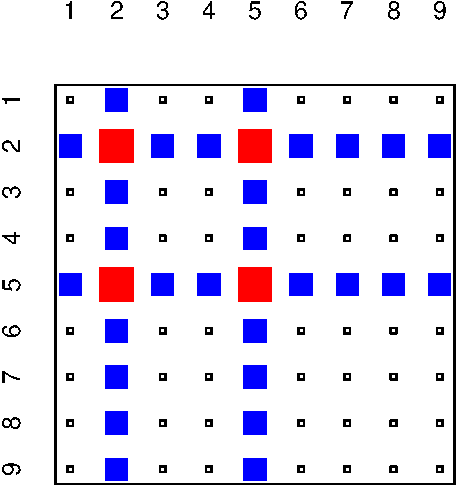
\includegraphics{wJacobi_files/figure-latex/figjacobi-1} \end{center}

Trigonometry

\(\alpha=\sin(\theta)\) and \(\beta=\cos(\theta)\)

\section{The Sequence}\label{the-sequence}

The \emph{strategy}

\section{Majorization}\label{majorization}

\begin{multline}
\sigma(y_1,\cdots,y_p)=\sigma(x_1+(y_1-x_1),\cdots,x_p+(y_p-x_p))\leq\\
\sigma(x_1,\cdots,x_p)+\sum_{s=1}^p(y_s-x_s)'\mathcal{D}_s\sigma(x_1,\cdots,x_p)+\\
\frac12\max_{0\leq\theta\leq 1}\sum_{s=1}^p\sum_{t=1}^p (y_s-x_s)'\{\mathcal{D}_{st}\sigma(x_1+\theta(x_1-y_1),\cdots,x_p+\theta(x_p-y_p))\}(y_t-x_t).
\end{multline}

\section{Applications}\label{applications}

\subsection{Symmetric Matrices}\label{symmetric-matrices}

All eigenvalues
Some eigenvalues

\subsection{Pairs of Matrices}\label{pairs-of-matrices}

\subsection{Rectangular Matrices}\label{rectangular-matrices}

\subsection{Simultaneous Diagonalization}\label{simultaneous-diagonalization}

\subsection{DMCA}\label{dmca}

\subsection{GCCA}\label{gcca}

\section{Appendix: Code}\label{appendix-code}

\subsection{pattern.R}\label{pattern.r}

\begin{Shaded}
\begin{Highlighting}[]
\NormalTok{mPrint }\OtherTok{\textless{}{-}} \ControlFlowTok{function}\NormalTok{(x,}
                   \AttributeTok{digits =} \DecValTok{6}\NormalTok{,}
                   \AttributeTok{width =} \DecValTok{8}\NormalTok{,}
                   \AttributeTok{format =} \StringTok{"f"}\NormalTok{,}
                   \AttributeTok{flag =} \StringTok{"+"}\NormalTok{) \{}
  \FunctionTok{print}\NormalTok{(}\FunctionTok{noquote}\NormalTok{(}
    \FunctionTok{formatC}\NormalTok{(}
\NormalTok{      x,}
      \AttributeTok{digits =}\NormalTok{ digits,}
      \AttributeTok{width =}\NormalTok{ width,}
      \AttributeTok{format =}\NormalTok{ format,}
      \AttributeTok{flag =}\NormalTok{ flag}
\NormalTok{    )}
\NormalTok{  ))}
\NormalTok{\}}

\NormalTok{butLast }\OtherTok{\textless{}{-}} \ControlFlowTok{function}\NormalTok{(x, }\AttributeTok{m =} \DecValTok{1}\NormalTok{) \{}
  \FunctionTok{return}\NormalTok{(}\FunctionTok{rev}\NormalTok{(}\FunctionTok{rev}\NormalTok{(x)[}\SpecialCharTok{{-}}\NormalTok{(}\DecValTok{1}\SpecialCharTok{:}\NormalTok{m)]))}
\NormalTok{\}}

\NormalTok{butFirst }\OtherTok{\textless{}{-}} \ControlFlowTok{function}\NormalTok{(x, }\AttributeTok{m =} \DecValTok{1}\NormalTok{) \{}
  \FunctionTok{return}\NormalTok{(x[}\SpecialCharTok{{-}}\NormalTok{(}\DecValTok{1}\SpecialCharTok{:}\NormalTok{m)])}
\NormalTok{\}}
\end{Highlighting}
\end{Shaded}

\section*{References}\label{references}
\addcontentsline{toc}{section}{References}

\phantomsection\label{refs}
\begin{CSLReferences}{1}{0}
\bibitem[\citeproctext]{ref-deleeuw_E_17o}
De Leeuw, J. 2017. {``{Jacobi Eigen in R/C with Lower Triangular Column-wise Compact Storage}.''} 2017. \url{https://jansweb.netlify.app/publication/deleeuw-e-17-o/deleeuw-e-17-o.pdf}.

\bibitem[\citeproctext]{ref-deleeuw_E_18g}
---------. 2018. {``{Simultaneous Diagonalization in R/C}.''} 2018. \url{https://jansweb.netlify.app/publication/deleeuw-e-18-g/deleeuw-e-18-g.pdf}.

\bibitem[\citeproctext]{ref-deleeuw_ferrari_R_08a}
De Leeuw, J., and D. B. Ferrari. 2008. {``{Using Jacobi Plane Rotations in R}.''} Preprint Series 556. Los Angeles, CA: UCLA Department of Statistics. \url{https://jansweb.netlify.app/publication/deleeuw-ferrari-r-08-a/deleeuw-ferrari-r-08-a.pdf}.

\bibitem[\citeproctext]{ref-deleeuw_pruzansky_A_78}
De Leeuw, J., and S. Pruzansky. 1978. {``A New Computational Method to Fit the Weighted Euclidean Distance Model.''} \emph{Psychometrika} 43: 479--90.

\bibitem[\citeproctext]{ref-gilbert_varadhan_19}
Gilbert, P., and R. Varadhan. 2019. \emph{{numDeriv: Accurate Numerical Derivatives}}. \url{https://CRAN.R-project.org/package=numDeriv}.

\bibitem[\citeproctext]{ref-jacobi_46}
Jacobi, C. G. J. 1846. {``{{Ü}ber ein leichtes Verfahren die in der Theorie der Sec{ü}larst{ö}rungen vorkommenden Gleichungen numerisch aufzul{ö}sen}.''} \emph{Journal f{ü}r Die Reine Und Angewandte Mathematik (Crelle's Journal)} 30: 51--94.

\end{CSLReferences}

\end{document}
